% Seção do estudo dos níveis de refinamento (niveis.py). Números: secoes/refino_niveis_valores.tex, tabelas e
% figuras niv_*, todos gerados por analise_niveis.py (rodar de novo atualiza o texto).
\IfFileExists{secoes/refino_niveis_valores.tex}{%% gerado por analise_niveis.py: os numeros citados em refino_niveis.tex
\def\nivAreaF{5,0}
\def\nivAreaG{15,7}
\def\nivBFMax{$-$0,25}
\def\nivBFMed{$-$0,93}
\def\nivBFMin{$-$1,89}
\def\nivBGMax{0,42}
\def\nivBGMed{$-$0,64}
\def\nivBGMin{$-$1,70}
\def\nivBXMax{$-$0,58}
\def\nivBXMed{$-$1,26}
\def\nivBXMin{$-$1,79}
\def\nivBzero{1,26}
\def\nivBzeroSinal{$-$1,26}
\def\nivCargaComp{3,5}
\def\nivCargaNova{2,9}
\def\nivCasos{det, r0, r1, r2, r3, r4, r5, r6, r7}
\def\nivCpuComp{15,1}
\def\nivCpuGI{1,0}
\def\nivCpuNova{10,8}
\def\nivCpuTriA{0,021}
\def\nivCpuTriD{0,114}
\def\nivCvCinco{4,1}
\def\nivCvCincoCont{4,9}
\def\nivCvMil{9,1}
\def\nivCvMilCont{11,0}
\def\nivDgaMax{1,08}
\def\nivDgbMax{1,10}
\def\nivDgcMax{0,57}
\def\nivDgcMed{0,06}
\def\nivDifEtapaUm{0}
\def\nivDpfZero{9,4}
\def\nivFACasosFora{0}
\def\nivFACel{105}
\def\nivFACpu{31,6}
\def\nivFACpuEq{31,6}
\def\nivFADist{0,23}
\def\nivFADpf{$-$16,9}
\def\nivFADpfAbs{16,9}
\def\nivFAEabs{2,55}
\def\nivFAEmax{4,26}
\def\nivFAEmed{$+$2,55}
\def\nivFAFora{0,00}
\def\nivFAForaMax{0,0}
\def\nivFAHcinco{0,74}
\def\nivFAHmil{0,15}
\def\nivFAMincinco{44}
\def\nivFAMinmil{9}
\def\nivFAPar{32,0}
\def\nivFAPf{8,97}
\def\nivFAR{2,94}
\def\nivFARcent{0,072}
\def\nivFARpct{7,2}
\def\nivFATri{998}
\def\nivFBCasosFora{0}
\def\nivFBCel{157}
\def\nivFBCpu{50,2}
\def\nivFBCpuEq{50,2}
\def\nivFBDist{0,17}
\def\nivFBDpf{$-$10,2}
\def\nivFBDpfAbs{10,2}
\def\nivFBEabs{1,49}
\def\nivFBEmax{2,52}
\def\nivFBEmed{$+$1,49}
\def\nivFBFora{0,00}
\def\nivFBForaMax{0,0}
\def\nivFBHcinco{1,17}
\def\nivFBHmil{0,23}
\def\nivFBMincinco{70}
\def\nivFBMinmil{14}
\def\nivFBPar{50,7}
\def\nivFBPf{9,70}
\def\nivFBR{4,66}
\def\nivFBRcent{0,115}
\def\nivFBRpct{11,5}
\def\nivFBTri{1385}
\def\nivFCCasosFora{0}
\def\nivFCCel{225}
\def\nivFCCpu{186,0}
\def\nivFCCpuEq{132,0}
\def\nivFCDist{0,16}
\def\nivFCDpf{$-$1,0}
\def\nivFCDpfAbs{1,0}
\def\nivFCEabs{0,23}
\def\nivFCEmax{0,49}
\def\nivFCEmaxS{$+$0,49}
\def\nivFCEmed{$+$0,14}
\def\nivFCEminS{$-$0,21}
\def\nivFCFora{0,00}
\def\nivFCForaMax{0,0}
\def\nivFCHcinco{3,09}
\def\nivFCHmil{0,62}
\def\nivFCMincinco{185}
\def\nivFCMinmil{37}
\def\nivFCPar{192,7}
\def\nivFCPf{10,69}
\def\nivFCR{12,27}
\def\nivFCRcent{0,302}
\def\nivFCRpct{30,2}
\def\nivFCTri{2385}
\def\nivFermiFoco{3,0}
\def\nivFermiHcincoFA{0,64}
\def\nivFermiHcincoFB{0,79}
\def\nivFermiHcincoFC{1,16}
\def\nivFermiHcincoFfixA{0,27}
\def\nivFermiHcincoFfixB{0,57}
\def\nivFermiHcincoFfixC{1,08}
\def\nivFermiHcincoFfixD{2,03}
\def\nivFermiHcincoGA{0,40}
\def\nivFermiHcincoGB{0,61}
\def\nivFermiHcincoGC{1,17}
\def\nivFermiHcincoGI{0,05}
\def\nivFermiHmilFA{0,13}
\def\nivFermiHmilFB{0,16}
\def\nivFermiHmilFC{0,23}
\def\nivFermiHmilFfixA{0,05}
\def\nivFermiHmilFfixB{0,11}
\def\nivFermiHmilFfixC{0,22}
\def\nivFermiHmilFfixD{0,41}
\def\nivFermiHmilGA{0,08}
\def\nivFermiHmilGB{0,12}
\def\nivFermiHmilGC{0,23}
\def\nivFermiHmilGI{0,01}
\def\nivFermiRazFA{0,32}
\def\nivFermiRazFB{0,39}
\def\nivFermiRazFC{0,57}
\def\nivFermiRazFfixA{0,13}
\def\nivFermiRazFfixB{0,28}
\def\nivFermiRazFfixC{0,54}
\def\nivFermiRazFfixD{1,00}
\def\nivFermiRazGA{0,20}
\def\nivFermiRazGB{0,30}
\def\nivFermiRazGC{0,58}
\def\nivFermiRazGI{0,02}
\def\nivFermiTFA{44}
\def\nivFermiTFB{54}
\def\nivFermiTFC{80}
\def\nivFermiTFfixA{19}
\def\nivFermiTFfixB{39}
\def\nivFermiTFfixC{75}
\def\nivFermiTFfixD{140}
\def\nivFermiTGA{28}
\def\nivFermiTGB{42}
\def\nivFermiTGC{81}
\def\nivFermiTGI{3}
\def\nivFermiTriFA{1718}
\def\nivFermiTriFB{2105}
\def\nivFermiTriFC{3105}
\def\nivFermiTriFfixA{720}
\def\nivFermiTriFfixB{1520}
\def\nivFermiTriFfixC{2906}
\def\nivFermiTriFfixD{5426}
\def\nivFermiTriGA{1081}
\def\nivFermiTriGB{1639}
\def\nivFermiTriGC{3135}
\def\nivFermiTriGI{126}
\def\nivFfixACasosFora{0}
\def\nivFfixACpu{15,1}
\def\nivFfixACpuEq{10,8}
\def\nivFfixADist{--}
\def\nivFfixADpf{$-$31,5}
\def\nivFfixADpfAbs{31,5}
\def\nivFfixAEabs{5,17}
\def\nivFfixAEmax{7,23}
\def\nivFfixAEmed{$+$5,17}
\def\nivFfixAFora{--}
\def\nivFfixAForaMax{--}
\def\nivFfixAHcinco{0,25}
\def\nivFfixAHmil{0,05}
\def\nivFfixAMincinco{15}
\def\nivFfixAMinmil{3}
\def\nivFfixAPar{15,5}
\def\nivFfixAPf{7,39}
\def\nivFfixAR{1,00}
\def\nivFfixARcent{0,025}
\def\nivFfixARpct{2,5}
\def\nivFfixATri{720}
\def\nivFfixBCasosFora{0}
\def\nivFfixBCpu{53,3}
\def\nivFfixBCpuEq{37,8}
\def\nivFfixBDist{--}
\def\nivFfixBDpf{$-$13,7}
\def\nivFfixBDpfAbs{13,7}
\def\nivFfixBEabs{2,04}
\def\nivFfixBEmax{3,21}
\def\nivFfixBEmed{$+$2,04}
\def\nivFfixBFora{--}
\def\nivFfixBForaMax{--}
\def\nivFfixBHcinco{0,89}
\def\nivFfixBHmil{0,18}
\def\nivFfixBMincinco{53}
\def\nivFfixBMinmil{11}
\def\nivFfixBPar{57,5}
\def\nivFfixBPf{9,32}
\def\nivFfixBR{3,52}
\def\nivFfixBRcent{0,086}
\def\nivFfixBRpct{8,6}
\def\nivFfixBTri{1520}
\def\nivFfixCCasosFora{0}
\def\nivFfixCCpu{179,7}
\def\nivFfixCCpuEq{127,6}
\def\nivFfixCDist{--}
\def\nivFfixCDpf{$-$10,8}
\def\nivFfixCDpfAbs{10,8}
\def\nivFfixCEabs{1,58}
\def\nivFfixCEmax{2,24}
\def\nivFfixCEmed{$+$1,58}
\def\nivFfixCFora{--}
\def\nivFfixCForaMax{--}
\def\nivFfixCHcinco{2,99}
\def\nivFfixCHmil{0,60}
\def\nivFfixCMincinco{179}
\def\nivFfixCMinmil{36}
\def\nivFfixCPar{184,5}
\def\nivFfixCPf{9,64}
\def\nivFfixCR{11,86}
\def\nivFfixCRcent{0,291}
\def\nivFfixCRpct{29,1}
\def\nivFfixCTri{2906}
\def\nivFfixDCasosFora{0}
\def\nivFfixDCpu{616,7}
\def\nivFfixDCpuEq{437,9}
\def\nivFfixDDist{--}
\def\nivFfixDDpf{0,0}
\def\nivFfixDDpfAbs{0,0}
\def\nivFfixDEabs{0,00}
\def\nivFfixDEmax{0,00}
\def\nivFfixDEmed{$+$0,00}
\def\nivFfixDFora{--}
\def\nivFfixDForaMax{--}
\def\nivFfixDHcinco{10,25}
\def\nivFfixDHmil{2,05}
\def\nivFfixDMincinco{615}
\def\nivFfixDMinmil{123}
\def\nivFfixDPar{634,4}
\def\nivFfixDPf{10,80}
\def\nivFfixDR{40,70}
\def\nivFfixDRcent{1,000}
\def\nivFfixDRpct{100,0}
\def\nivFfixDTri{5426}
\def\nivGACasosFora{9}
\def\nivGACel{49}
\def\nivGACpu{20,0}
\def\nivGACpuEq{20,0}
\def\nivGADist{0,51}
\def\nivGADpf{$-$16,3}
\def\nivGADpfAbs{16,3}
\def\nivGAEabs{2,46}
\def\nivGAEmax{3,84}
\def\nivGAEmed{$+$2,46}
\def\nivGAFora{3,65}
\def\nivGAForaMax{6,0}
\def\nivGAHcinco{0,47}
\def\nivGAHmil{0,09}
\def\nivGAMincinco{28}
\def\nivGAMinmil{6}
\def\nivGAPar{20,2}
\def\nivGAPf{9,03}
\def\nivGAR{1,86}
\def\nivGARcent{0,046}
\def\nivGARpct{4,6}
\def\nivGATri{955}
\def\nivGBCasosFora{9}
\def\nivGBCel{49}
\def\nivGBCpu{47,0}
\def\nivGBCpuEq{47,0}
\def\nivGBDist{0,47}
\def\nivGBDpf{$-$8,7}
\def\nivGBDpfAbs{8,7}
\def\nivGBEabs{1,26}
\def\nivGBEmax{1,64}
\def\nivGBEmed{$+$1,26}
\def\nivGBFora{4,55}
\def\nivGBForaMax{5,8}
\def\nivGBHcinco{1,10}
\def\nivGBHmil{0,22}
\def\nivGBMincinco{66}
\def\nivGBMinmil{13}
\def\nivGBPar{47,7}
\def\nivGBPf{9,86}
\def\nivGBR{4,37}
\def\nivGBRcent{0,107}
\def\nivGBRpct{10,7}
\def\nivGBTri{1513}
\def\nivGCCasosFora{8}
\def\nivGCCel{49}
\def\nivGCCpu{180,8}
\def\nivGCCpuEq{180,8}
\def\nivGCDist{0,45}
\def\nivGCDpf{$-$1,4}
\def\nivGCDpfAbs{1,4}
\def\nivGCEabs{0,32}
\def\nivGCEmax{0,85}
\def\nivGCEmed{$+$0,20}
\def\nivGCFora{1,67}
\def\nivGCForaMax{3,7}
\def\nivGCHcinco{4,23}
\def\nivGCHmil{0,85}
\def\nivGCMincinco{254}
\def\nivGCMinmil{51}
\def\nivGCPar{183,3}
\def\nivGCPf{10,64}
\def\nivGCR{16,81}
\def\nivGCRcent{0,413}
\def\nivGCRpct{41,3}
\def\nivGCTri{3009}
\def\nivGICasosFora{0}
\def\nivGICpu{1,0}
\def\nivGICpuEq{1,0}
\def\nivGIDist{--}
\def\nivGIDpf{$-$88,0}
\def\nivGIDpfAbs{88,0}
\def\nivGIEabs{26,87}
\def\nivGIEmax{37,42}
\def\nivGIEmed{$+$26,87}
\def\nivGIFora{--}
\def\nivGIForaMax{--}
\def\nivGIHcinco{0,02}
\def\nivGIHmil{0,00}
\def\nivGIMincinco{1}
\def\nivGIMinmil{0}
\def\nivGIPar{1,0}
\def\nivGIPf{1,29}
\def\nivGIR{0,09}
\def\nivGIRcent{0,002}
\def\nivGIRpct{0,2}
\def\nivGITri{126}
\def\nivMln{0,3475}
\def\nivNcasos{9}
\def\nivNcasosEtapaUm{9}
\def\nivPFMax{2,30}
\def\nivPFMed{1,36}
\def\nivPFMin{0,28}
\def\nivPFN{4}
\def\nivPGMax{5,38}
\def\nivPGMed{2,20}
\def\nivPGMin{0,39}
\def\nivPGN{6}
\def\nivPXMax{0,50}
\def\nivPXMed{0,50}
\def\nivPXMin{0,50}
\def\nivPXN{1}
\def\nivParComp{15,5}
\def\nivParNova{10,9}
\def\nivPfCont{7,60}
\def\nivPfLn{7,39}
\def\nivPfRef{10,80}
\def\nivPfZero{11,81}
\def\nivQuedaF{7}
\def\nivQuedaG{6}
\def\nivQuedaX{8}
\def\nivRazEtapa{0,71}
\def\nivRazEtapaGF{11}
\def\nivRazEtapaMax{0,73}
\def\nivRazEtapaMin{0,67}
\def\nivSemSolF{5}
\def\nivSemSolG{3}
\def\nivSemSolX{8}
\def\nivSensPf{7,2}
\def\nivSln{0,2401}
}{}

\section{Níveis de refinamento e malha inicial}\label{sec:ref:niveis}

O refinamento por realização da Seção~\ref{sec:ref:metodo} tem três escolhas em aberto: o tamanho $h$ dos elementos em
volta da banda, a malha inicial da etapa~1 (que só precisa localizar a banda) e o número de passos de refinamento.
Esta seção mede o erro e o custo de cada escolha nos mesmos casos da comparação
(Seção~\ref{sec:ref:comparacao}) para decidir a configuração do Monte Carlo no \emph{cluster} fermi.

\subsection{Desenho do estudo}\label{sec:ref:niveis:desenho}

\paragraph{Modelo e casos.} O exemplo saturado do Ceron, exatamente como na comparação (GIM com
\emph{arc-length} em $t = 0{,}01$\,h, \emph{solver} \emph{skyline} com uma \emph{thread}), no caso determinístico
(det) e nas realizações 0 a 7 (r0 a r7) da semente padrão: nove casos.

\paragraph{Malhas iniciais.} Duas malhas para a etapa~1, com o mesmo contorno, os mesmos grupos físicos e, portanto, o
mesmo retângulo do Karhunen--Loève e o mesmo campo aleatório de cada realização
(Figura~\ref{fig:niv:malhas_iniciais}):
\begin{itemize}
  \item \textbf{foco375} (720 triângulos): 0,375\,m na região ocupada pelas bandas de 33 rodadas anteriores, 0,9\,m na
        superfície e 3\,m no fundo; é a malha da fase~1 no fermi e a etapa~1 da comparação;
  \item \textbf{g15} (126 triângulos): $h_\text{sup} = 1{,}5$\,m na superfície e $h_\text{max} = 3$\,m, sem foco.
\end{itemize}

\paragraph{Níveis.} De cada malha inicial, um passo de refinamento a partir da banda da etapa~1
(\texttt{refina\_\allowbreak banda.py}, folga 0,375\,m e limiar 0,1), com $h = 0{,}25$, $0{,}1875$ e $0{,}125$\,m; a malha refinada
mantém os campos de tamanho da malha inicial fora da banda. A configuração foco375 $\to$ 0,125 é a ``refinada'' da
comparação e não foi rodada de novo (marcada com $^{*}$ nas tabelas). As malhas dos níveis estão nas
Figuras~\ref{fig:niv:niveis_det}, \ref{fig:niv:niveis_r3}, \ref{fig:niv:niveis_r5} e~\ref{fig:niv:niveis_r7}. As
malhas fixas da comparação (foco375, foco25, foco1875 e foco125, com 0,375, 0,25, 0,1875 e 0,125\,m no foco) entram
como termo de comparação.

\paragraph{Execução e custo.} O \texttt{niveis.py} roda uma fila com três processos ao mesmo tempo
(\texttt{PARALELO=3}, numa máquina de quatro núcleos), com um executável congelado. O custo de uma configuração num
caso é o da cadeia: a etapa~1, o \texttt{refina\_\allowbreak banda.py} (com o \texttt{gmsh}) e a rodada refinada, em tempo de
parede e em tempo de CPU (usuário + sistema). A comparação rodou com \texttt{PARALELO=2}, outro \emph{build} do
programa e mais carga na máquina (carga média de 1\,min de \nivCargaComp{} contra \nivCargaNova{} nesta campanha). A
Tabela~\ref{tab:niv:etapa1} confere as duas campanhas na mesma rodada, a foco375 da etapa~1: o fator de segurança é
o mesmo nos \nivNcasosEtapaUm{} casos (diferença relativa máxima \nivDifEtapaUm), mas o CPU desta campanha é
\nivRazEtapa{} vezes o da comparação (de \nivRazEtapaMin{} a \nivRazEtapaMax{} por caso). Por isso o custo é
comparado dentro de cada campanha: $R$ é o CPU médio da cadeia dividido pelo CPU médio da foco375 da mesma campanha, e
o ``CPU equivalente'' das figuras é $R$ vezes o CPU médio da foco375 desta campanha (\nivCpuNova\,s). Essa
normalização supõe que a diferença entre as campanhas é a mesma para as rodadas maiores; é uma aproximação. Os
custos locais são os do \emph{solver} \emph{skyline}, cujo custo cresce mais que linearmente com a malha (na
comparação, \nivCpuTriA\,s de CPU por triângulo na foco375 e \nivCpuTriD\,s na foco125); no fermi, com o PARDISO, o
tempo é quase linear nos triângulos, e as razões de custo locais não valem lá
(Seção~\ref{sec:ref:niveis:recomendacao}).

\begin{table}[H]
  \centering\small
  \caption{Tempo de CPU (s) da rodada foco375 da etapa~1 nas duas campanhas (mesma malha e mesmo modelo).}
  \label{tab:niv:etapa1}
  \begin{tabular}{@{}l rrrr r@{}}
\toprule
CPU (s) & \multicolumn{1}{c}{det} & \multicolumn{1}{c}{r0} & \multicolumn{1}{c}{r1} & \multicolumn{1}{c}{r2} & média \\
\midrule
nova (\texttt{PARALELO=3}) & 11{,}20 & 8{,}91 & 10{,}44 & 10{,}00 & 10{,}14 \\
comparação (\texttt{PARALELO=2}) & 15{,}54 & 12{,}67 & 14{,}23 & 14{,}16 & 14{,}15 \\
razão nova/comparação & 0{,}721 & 0{,}703 & 0{,}734 & 0{,}706 & 0{,}716 \\
\bottomrule
\end{tabular}

\end{table}

\paragraph{Referência.} O erro de cada configuração é $e = \Gamma/\Gamma_\text{foco125} - 1$, com a foco125 fixa
(5426 triângulos) do mesmo caso. A foco125 não está convergida: a refinada da comparação, também com 0,125\,m na
banda, difere dela de \nivFCEminS\,\% a \nivFCEmaxS\,\% nos casos usados aqui, e a referência mais fina prevista no \texttt{niveis.py}
($h = 0{,}0625$\,m) foi cortada para economizar tempo. Assim, $e$ mede a distância até a foco125, não até a solução
exata; a Seção~\ref{sec:ref:niveis:conv} estima essa distância por extrapolação.

\paragraph{Casos usados.} A campanha terminou com as 63 rodadas feitas, sem falhas nem rodadas sem banda; os
resultados a seguir usam os casos com todas as configurações: \nivCasos{} (\nivNcasos{} casos).

\subsection{Erro e custo}\label{sec:ref:niveis:resultados}

A Tabela~\ref{tab:niv:resumo} resume cada configuração e a Tabela~\ref{tab:niv:casos} dá $\Gamma$ e $e$ por caso. Nas
duas cadeias o erro cai com $h$ e, em $h = 0{,}25$ e $0{,}1875$, é positivo em todos os casos (a malha mais grossa
superestima $\Gamma$): $\overline{|e|}$ vai de
\nivFAEabs\,\% ($h = 0{,}25$) a \nivFBEabs\,\% ($0{,}1875$) e \nivFCEabs\,\% ($0{,}125$) na cadeia da foco375 e de
\nivGAEabs\,\% a \nivGBEabs\,\% e \nivGCEabs\,\% na da g15. Com o mesmo $h$, as duas malhas iniciais dão erros médios
parecidos, mas os fatores das duas cadeias diferem caso a caso em até \nivDgaMax\,\%, \nivDgbMax\,\% e
\nivDgcMax\,\% em $h = 0{,}25$, $0{,}1875$ e $0{,}125$. A g15 sozinha erra muito ($\bar e = $ \nivGIEmed\,\%), mas serve para localizar a banda.

\begin{table}[H]
  \centering\footnotesize
  \setlength{\tabcolsep}{4pt}
  \caption{Resumo por configuração: triângulos (média), erro em relação à foco125 ($\overline{|e|}$, $\max|e|$ e
  $\bar e$, com sinal), tempos médios da cadeia por caso (CPU e parede, sem normalizar), custo relativo à foco125
  ($R/R_{125}$, CPU normalizado pela foco375 de cada campanha) e contenção da banda (a maior distância $d_{\max}$ dos
  pontos da banda da rodada refinada aos pontos da banda que fizeram a malha dela, e a fração média dos pontos a mais
  de 0,375\,m). $^{*}$: a refinada da comparação (\texttt{PARALELO=2}).}
  \label{tab:niv:resumo}
  \begin{tabular}{@{}l r r r r r r r r r@{}}
\toprule
 & & \multicolumn{3}{c}{$e$ (\%)} & \multicolumn{3}{c}{custo da cadeia por caso} & \multicolumn{2}{c}{contenção da banda} \\
\cmidrule(lr){3-5}\cmidrule(lr){6-8}\cmidrule(l){9-10}
Configuração & triâng. & $\overline{|e|}$ & $\max|e|$ & $\bar e$ & CPU (s) & parede (s) & $R/R_{125}$ & $d_{\max}$ (m) & fora (\%) \\
\midrule
foco375 (fixa) & 720 & 5{,}17 & 7{,}23 & $+$5{,}17 & 15{,}1 & 15{,}5 & 0{,}025 & -- & -- \\
foco25 (fixa) & 1520 & 2{,}04 & 3{,}21 & $+$2{,}04 & 53{,}3 & 57{,}5 & 0{,}086 & -- & -- \\
foco1875 (fixa) & 2906 & 1{,}58 & 2{,}24 & $+$1{,}58 & 179{,}7 & 184{,}5 & 0{,}291 & -- & -- \\
foco125 (fixa, ref.) & 5426 & -- & -- & -- & 616{,}7 & 634{,}4 & 1{,}000 & -- & -- \\
\midrule
foco375 $\to$ 0,25 & 998 & 2{,}55 & 4{,}26 & $+$2{,}55 & 31{,}6 & 32{,}0 & 0{,}072 & 0{,}234 & 0{,}00 \\
foco375 $\to$ 0,1875 & 1385 & 1{,}49 & 2{,}52 & $+$1{,}49 & 50{,}2 & 50{,}7 & 0{,}115 & 0{,}174 & 0{,}00 \\
foco375 $\to$ 0,125$^{*}$ & 2385 & 0{,}23 & 0{,}49 & $+$0{,}14 & 186{,}0 & 192{,}7 & 0{,}302 & 0{,}159 & 0{,}00 \\
\midrule
g15 (só etapa 1) & 126 & 26{,}87 & 37{,}42 & $+$26{,}87 & 1{,}0 & 1{,}0 & 0{,}002 & -- & -- \\
g15 $\to$ 0,25 & 955 & 2{,}46 & 3{,}84 & $+$2{,}46 & 20{,}0 & 20{,}2 & 0{,}046 & 0{,}508 & 3{,}65 \\
g15 $\to$ 0,1875 & 1513 & 1{,}26 & 1{,}64 & $+$1{,}26 & 47{,}0 & 47{,}7 & 0{,}107 & 0{,}475 & 4{,}55 \\
g15 $\to$ 0,125 & 3009 & 0{,}32 & 0{,}85 & $+$0{,}20 & 180{,}8 & 183{,}3 & 0{,}413 & 0{,}455 & 1{,}67 \\
\bottomrule
\end{tabular}

\end{table}

\begin{table}[H]
  \centering\footnotesize
  \setlength{\tabcolsep}{3.5pt}
  \caption{Fator de segurança $\Gamma$ por caso e configuração e a diferença $e$ para a foco125.}
  \label{tab:niv:casos}
  \begin{tabular}{@{}l rrrrrrrrr@{}}
\toprule
Configuração & \multicolumn{1}{c}{det} & \multicolumn{1}{c}{r0} & \multicolumn{1}{c}{r1} & \multicolumn{1}{c}{r2} & \multicolumn{1}{c}{r3} & \multicolumn{1}{c}{r4} & \multicolumn{1}{c}{r5} & \multicolumn{1}{c}{r6} & \multicolumn{1}{c}{r7} \\
\midrule
foco375 (fixa) & 1{,}4633 & 1{,}1224 & 1{,}4171 & 1{,}1731 & 1{,}9124 & 1{,}4702 & 0{,}9544 & 1{,}5654 & 1{,}1116 \\
foco25 (fixa) & 1{,}4210 & 1{,}0883 & 1{,}3889 & 1{,}1360 & 1{,}8688 & 1{,}4095 & 0{,}9216 & 1{,}5067 & 1{,}0896 \\
foco1875 (fixa) & 1{,}4138 & 1{,}0845 & 1{,}3851 & 1{,}1298 & 1{,}8554 & 1{,}4036 & 0{,}9184 & 1{,}4897 & 1{,}0918 \\
foco125 (fixa, ref.) & 1{,}3910 & 1{,}0667 & 1{,}3660 & 1{,}1051 & 1{,}8395 & 1{,}3767 & 0{,}9030 & 1{,}4599 & 1{,}0840 \\
\midrule
foco375 $\to$ 0,25 & 1{,}4222 & 1{,}0947 & 1{,}3947 & 1{,}1424 & 1{,}8763 & 1{,}4153 & 0{,}9271 & 1{,}5221 & 1{,}0940 \\
foco375 $\to$ 0,1875 & 1{,}4101 & 1{,}0823 & 1{,}3865 & 1{,}1263 & 1{,}8559 & 1{,}4030 & 0{,}9129 & 1{,}4967 & 1{,}0916 \\
foco375 $\to$ 0,125$^{*}$ & 1{,}3976 & 1{,}0644 & 1{,}3727 & 1{,}1029 & 1{,}8413 & 1{,}3787 & 0{,}9037 & 1{,}4642 & 1{,}0852 \\
\midrule
g15 (só etapa 1) & 1{,}7444 & 1{,}3484 & 1{,}6119 & 1{,}4338 & 2{,}2658 & 1{,}8459 & 1{,}1560 & 2{,}0062 & 1{,}2965 \\
g15 $\to$ 0,25 & 1{,}4200 & 1{,}0958 & 1{,}3954 & 1{,}1475 & 1{,}8748 & 1{,}4209 & 0{,}9172 & 1{,}5131 & 1{,}0952 \\
g15 $\to$ 0,1875 & 1{,}4073 & 1{,}0841 & 1{,}3850 & 1{,}1223 & 1{,}8616 & 1{,}3904 & 0{,}9122 & 1{,}4802 & 1{,}0944 \\
g15 $\to$ 0,125 & 1{,}3916 & 1{,}0705 & 1{,}3726 & 1{,}1044 & 1{,}8418 & 1{,}3804 & 0{,}8986 & 1{,}4723 & 1{,}0866 \\
\midrule
\multicolumn{10}{@{}l}{\emph{Diferença para a foco125, $e$ (\%)}} \\
foco375 (fixa) & $+$5{,}20 & $+$5{,}22 & $+$3{,}74 & $+$6{,}15 & $+$3{,}96 & $+$6{,}79 & $+$5{,}70 & $+$7{,}23 & $+$2{,}54 \\
foco25 (fixa) & $+$2{,}15 & $+$2{,}02 & $+$1{,}67 & $+$2{,}80 & $+$1{,}59 & $+$2{,}38 & $+$2{,}06 & $+$3{,}21 & $+$0{,}51 \\
foco1875 (fixa) & $+$1{,}64 & $+$1{,}66 & $+$1{,}40 & $+$2{,}24 & $+$0{,}86 & $+$1{,}95 & $+$1{,}70 & $+$2{,}04 & $+$0{,}72 \\
foco375 $\to$ 0,25 & $+$2{,}24 & $+$2{,}63 & $+$2{,}10 & $+$3{,}37 & $+$2{,}00 & $+$2{,}80 & $+$2{,}67 & $+$4{,}26 & $+$0{,}92 \\
foco375 $\to$ 0,1875 & $+$1{,}37 & $+$1{,}46 & $+$1{,}50 & $+$1{,}92 & $+$0{,}89 & $+$1{,}91 & $+$1{,}10 & $+$2{,}52 & $+$0{,}70 \\
foco375 $\to$ 0,125$^{*}$ & $+$0{,}47 & $-$0{,}21 & $+$0{,}49 & $-$0{,}20 & $+$0{,}09 & $+$0{,}14 & $+$0{,}08 & $+$0{,}29 & $+$0{,}11 \\
g15 (só etapa 1) & $+$25{,}40 & $+$26{,}41 & $+$18{,}00 & $+$29{,}75 & $+$23{,}17 & $+$34{,}08 & $+$28{,}01 & $+$37{,}42 & $+$19{,}60 \\
g15 $\to$ 0,25 & $+$2{,}08 & $+$2{,}72 & $+$2{,}15 & $+$3{,}84 & $+$1{,}92 & $+$3{,}21 & $+$1{,}57 & $+$3{,}65 & $+$1{,}03 \\
g15 $\to$ 0,1875 & $+$1{,}17 & $+$1{,}64 & $+$1{,}39 & $+$1{,}56 & $+$1{,}20 & $+$0{,}99 & $+$1{,}02 & $+$1{,}39 & $+$0{,}95 \\
g15 $\to$ 0,125 & $+$0{,}04 & $+$0{,}35 & $+$0{,}48 & $-$0{,}06 & $+$0{,}12 & $+$0{,}27 & $-$0{,}49 & $+$0{,}85 & $+$0{,}24 \\
\bottomrule
\end{tabular}

\end{table}

A Figura~\ref{fig:niv:erro_tempo} põe o erro contra o custo. Com o mesmo $h$ na banda, a malha refinada por
realização tem erro próximo ao da malha fixa. Em $h = 0{,}25$ o ganho é pequeno: foco375 $\to$ 0,25 custa
$R/R_{125} = $ \nivFARcent{} contra \nivFfixBRcent{} da foco25, com erro um pouco maior
($\overline{|e|} = $ \nivFAEabs\,\% contra \nivFfixBEabs\,\%). A vantagem aparece nos níveis finos, em que a malha
fixa refina todo o foco: foco375 $\to$ 0,1875 custa \nivFBRcent{} contra \nivFfixCRcent{} da foco1875, e
foco375 $\to$ 0,125 custa \nivFCRcent{} da foco125, com $\overline{|e|} = $ \nivFCEabs\,\% e
$\max|e| = $ \nivFCEmax\,\%. A Figura~\ref{fig:niv:etapas} separa o custo por
etapa: a rodada refinada domina, e o \texttt{refina\_\allowbreak banda.py} com o \texttt{gmsh} é desprezível. A etapa~1 da g15 é
cerca de \nivRazEtapaGF{} vezes mais barata que a da foco375 (\nivCpuGI\,s contra \nivCpuNova\,s de CPU), mas em $h = 0{,}125$ a malha refinada da g15 é maior
(\nivGCTri{} contra \nivFCTri{} triângulos em média), porque a banda localizada com elementos de 1,5\,m
ocupa uma faixa mais larga (área média da banda na etapa~1 de \nivAreaG\,m$^2$ contra \nivAreaF\,m$^2$, embora com
menos pontos: \nivGCCel{} contra \nivFCCel), e a cadeia sai mais cara: CPU equivalente de \nivGCCpuEq\,s
contra \nivFCCpuEq\,s.

\begin{figure}[H]
  \centering
  \includegraphics[width=\textwidth]{niv_erro_tempo}
  \caption{Erro médio e máximo em relação à foco125 contra o CPU médio da cadeia por caso (eixos logarítmicos; CPU na
  escala desta campanha, a comparação multiplicada por \nivRazEtapa). Cinza: malhas fixas; azul: foco375 $\to h$;
  laranja: g15 $\to h$ (triângulo vazado: a g15 sozinha). A linha pontilhada marca o custo da foco125.}
  \label{fig:niv:erro_tempo}
\end{figure}

\begin{figure}[H]
  \centering
  \includegraphics[width=\textwidth]{niv_etapas}
  \caption{CPU médio por caso de cada etapa da cadeia (escala desta campanha): etapa~1 na malha inicial,
  \texttt{refina\_\allowbreak banda.py} com o \texttt{gmsh} e rodada refinada. Na refinada da comparação, as etapas vêm do CPU da
  cadeia repartido pelos tempos de parede de cada etapa.}
  \label{fig:niv:etapas}
\end{figure}

\paragraph{Contenção da banda.} Na cadeia da foco375 a banda da rodada refinada fica toda dentro da região refinada:
$d_{\max}$ não passa de \nivFADist\,m, \nivFBDist\,m e \nivFCDist\,m (para $h = 0{,}25$, $0{,}1875$ e $0{,}125$) e
nenhum ponto passa da folga. Na cadeia da g15 a banda refinada sai da região refinada: $d_{\max}$ chega a
\nivGADist\,m, \nivGBDist\,m e \nivGCDist\,m, acima da folga de 0,375\,m, com até \nivGAForaMax\,\%,
\nivGBForaMax\,\% e \nivGCForaMax\,\% dos pontos da banda fora dela num caso
(Figura~\ref{fig:niv:contencao}). A banda localizada com elementos de 1,5\,m é deslocada em relação à verdadeira; a
coincidência de $\Gamma$ com a cadeia da foco375 nestes casos não garante o mesmo em todas as realizações.

\begin{figure}[H]
  \centering
  \includegraphics[width=\textwidth]{niv_contencao}
  \caption{Contenção da banda: a maior distância $d_{\max}$ dos pontos da banda de cada rodada refinada aos pontos da
  banda com que a malha dela foi feita (os pontos do \texttt{.geo}), por caso. Linha tracejada: a folga de 0,375\,m.}
  \label{fig:niv:contencao}
\end{figure}

\subsection{Convergência e extrapolação}\label{sec:ref:niveis:conv}

A Figura~\ref{fig:niv:convergencia} mostra $\Gamma/\Gamma_\text{foco125} - 1$ contra $h$ em cada caso, nas duas
cadeias e nas malhas fixas. Com três níveis ($h_1, h_2, h_3$) = (0,25; 0,1875; 0,125)\,m de cada cadeia, o modelo
$\Gamma(h) = \Gamma_0 + C h^p$ dá $p$ pela razão
$(\Gamma_1 - \Gamma_2)/(\Gamma_2 - \Gamma_3) = (h_1^p - h_2^p)/(h_2^p - h_3^p)$. Como os dois passos têm o mesmo
$\Delta h = 0{,}0625$\,m, uma queda maior no segundo passo (razão menor que 1) implica $p < 1$, e uma razão menor que
0,71 (o limite para $p \to 0$) não tem solução com $p > 0$. Os ajustes são erráticos (Tabela~\ref{tab:niv:extrap}): a
queda de 0,1875 para 0,125 é maior que a de 0,25 para 0,1875 em \nivQuedaF{} dos \nivNcasos{} casos na cadeia da
foco375, em \nivQuedaG{} na da g15 e em \nivQuedaX{} nas malhas fixas; não há solução com $0{,}05 < p < 12$ (ou a
sequência não é monótona) em \nivSemSolF, \nivSemSolG{} e \nivSemSolX{} casos, respectivamente; nos casos com solução, $p$ vai
de \nivPFMin{} a \nivPFMax{} na cadeia da foco375 (\nivPFN{} casos) e de \nivPGMin{} a \nivPGMax{} na da g15
(\nivPGN{} casos); nas malhas fixas só r3 tem solução ($p = $ \nivPXMin). As malhas não estão no regime assintótico, e
os $p$ observados não servem para extrapolar. Com $p = 2$ como limite (com $p$ menor a correção seria maior), a
extrapolação pelos dois níveis mais finos, $\Gamma_0^{(2)} = \Gamma_3 - 0{,}8\,(\Gamma_2 - \Gamma_3)$, fica em média
\nivBFMed\,\% (cadeia foco375), \nivBGMed\,\% (g15) e \nivBXMed\,\% (malhas fixas) em relação à foco125. É uma
estimativa grosseira (malhas não aninhadas e só três níveis), mas indica que a própria foco125 superestima $\Gamma$ em
cerca de 1\,\%.

\begin{figure}[H]
  \centering
  \includegraphics[width=\textwidth]{niv_convergencia}
  \caption{$\Gamma/\Gamma_\text{foco125} - 1$ contra o tamanho $h$ na banda (ou no foco, nas malhas fixas), por caso.
  Em $h = 0$, os símbolos vazados são as extrapolações $\Gamma_0^{(2)}$ ($p = 2$) de cada cadeia.}
  \label{fig:niv:convergencia}
\end{figure}

\begin{table}[H]
  \centering\small
  \caption{Extrapolação por caso: a ordem observada $p$ (n.\,m.: sequência não monótona; $<0{,}05$: sem solução com
  $p > 0{,}05$) e $\Gamma_0^{(2)}/\Gamma_\text{foco125} - 1$ com $p = 2$, em \%. Na média de $p$, entre parênteses, o
  número de casos com solução.}
  \label{tab:niv:extrap}
  \begin{tabular}{@{}l r r r r r r@{}}
\toprule
 & \multicolumn{2}{c}{cadeia foco375} & \multicolumn{2}{c}{cadeia g15} & \multicolumn{2}{c}{malhas fixas} \\
\cmidrule(lr){2-3}\cmidrule(lr){4-5}\cmidrule(l){6-7}
Caso & $p$ & $\Gamma_0^{(2)}$ (\%) & $p$ & $\Gamma_0^{(2)}$ (\%) & $p$ & $\Gamma_0^{(2)}$ (\%) \\
\midrule
det & 0{,}88 & $-$0{,}25 & 0{,}39 & $-$0{,}86 & $<0{,}05$ & $-$1{,}31 \\
r0 & $<0{,}05$ & $-$1{,}55 & 0{,}53 & $-$0{,}67 & $<0{,}05$ & $-$1{,}33 \\
r2 & $<0{,}05$ & $-$1{,}89 & 2{,}04 & $-$1{,}35 & $<0{,}05$ & $-$1{,}79 \\
\midrule
média & 0{,}88$^{\,(1)}$ & $-$1{,}23 & 0{,}98 & $-$0{,}96 & -- & $-$1{,}48 \\
\bottomrule
\end{tabular}

\end{table}

\subsection{Consequência para a probabilidade de falha}\label{sec:ref:niveis:pf}

Na fase~1 no fermi (foco375, 1000 realizações) o fator teve média 1,457 e desvio 0,355 (CoV 24,4\,\%), com
$P_f = 7{,}60$\,\% por contagem. O ajuste lognormal tem $\mu_{\ln} = $ \nivMln{} e $\sigma_{\ln} = $ \nivSln{} e dá
$P_f = \Phi(-\mu_{\ln}/\sigma_{\ln}) = $ \nivPfLn\,\%. Se uma configuração X tem viés médio $b_X$ (o $\bar e$ da
Tabela~\ref{tab:niv:resumo}) e a foco375 tem $b_{375}$, então $\Gamma_X \approx \Gamma_{375}(1+b_X)/(1+b_{375})$ e
\begin{equation}
  P_{f,X} = \Phi\!\left(\frac{\ln(1+b_{375}) - \ln(1+b_X) - \mu_{\ln}}{\sigma_{\ln}}\right),
\end{equation}
que, na foco125 ($b_X = 0$), é $P_f = $ \nivPfRef\,\%. A Tabela~\ref{tab:niv:pf} compara o desvio de $P_f$ de cada
configuração com o coeficiente de variação do estimador de Monte Carlo, $\sqrt{(1-P_f)/(N P_f)}$: \nivCvMil\,\% com
$N = 1000$ e \nivCvCinco\,\% com $N = 5000$ (com $P_f = 7{,}60$\,\%, \nivCvMilCont\,\% e \nivCvCincoCont\,\%). Perto de
$P_f$, cada 1\,\% de viés em $\Gamma$ muda $P_f$ em cerca de \nivSensPf\,\%. Assim, o viés da foco375 da fase~1
($\bar e = $ \nivFfixAEmed\,\%) reduz $P_f$ em \nivFfixADpfAbs\,\%, e o de $h = 0{,}1875$ (\nivFBEmed\,\%) em
\nivFBDpfAbs\,\%, acima do erro de amostragem com $N = 5000$ e comparável ao de $N = 1000$; só $h = 0{,}125$ deixa o
viés (\nivFCDpfAbs\,\% em foco375 $\to$ 0,125 e \nivGCDpfAbs\,\% em g15 $\to$ 0,125) bem abaixo do erro de
amostragem. A última linha da tabela usa a extrapolação $\Gamma_0^{(2)}$ das malhas fixas como referência: o viés
residual da foco125 (\nivBzeroSinal\,\% em $\Gamma_0$) mudaria $P_f$ em \nivDpfZero\,\%, da ordem do erro de amostragem
com $N = 1000$.

\begin{table}[H]
  \centering\small
  \caption{Viés médio $\bar e$ em relação à foco125, $P_f$ resultante (lognormal da fase~1 corrigida pelo viés) e o
  desvio em relação a $P_f$ da foco125, comparados ao coeficiente de variação de Monte Carlo.}
  \label{tab:niv:pf}
  \begin{tabular}{@{}l r r r r@{}}
\toprule
Configuração & $\bar e$ (\%) & $P_f$ (\%) & $\Delta P_f$ (p.p.) & $\Delta P_f/P_f$ (\%) \\
\midrule
foco375 (fixa) & $+$5{,}08 & 7{,}39 & $-$3{,}34 & $-$31{,}1 \\
foco25 (fixa) & $+$2{,}16 & 9{,}18 & $-$1{,}56 & $-$14{,}5 \\
foco1875 (fixa) & $+$1{,}73 & 9{,}47 & $-$1{,}26 & $-$11{,}8 \\
foco125 (fixa, ref.) & $+$0{,}00 & 10{,}73 & $+$0{,}00 & $+$0{,}0 \\
\midrule
foco375 $\to$ 0,25 & $+$2{,}59 & 8{,}90 & $-$1{,}84 & $-$17{,}1 \\
foco375 $\to$ 0,1875 & $+$1{,}56 & 9{,}58 & $-$1{,}15 & $-$10{,}7 \\
foco375 $\to$ 0,125$^{*}$ & $+$0{,}14 & 10{,}62 & $-$0{,}11 & $-$1{,}0 \\
\midrule
g15 (só etapa 1) & $+$24{,}89 & 1{,}51 & $-$9{,}22 & $-$85{,}9 \\
g15 $\to$ 0,25 & $+$2{,}70 & 8{,}82 & $-$1{,}91 & $-$17{,}8 \\
g15 $\to$ 0,1875 & $+$1{,}44 & 9{,}67 & $-$1{,}06 & $-$9{,}9 \\
g15 $\to$ 0,125 & $+$0{,}20 & 10{,}57 & $-$0{,}16 & $-$1{,}5 \\
\midrule
$\Gamma_0$ estimado ($p = 2$, fixas) & $-$1{,}39 & 11{,}85 & $+$1{,}11 & $+$10{,}4 \\
\midrule
\multicolumn{5}{@{}l}{\emph{Coeficiente de variação de Monte Carlo de $P_f$ (com $P_f$ = 10{,}73\,\%)}} \\
$N = \num{1000}$ & \multicolumn{4}{r@{}}{9{,}1\,\%} \\
$N = \num{5000}$ & \multicolumn{4}{r@{}}{4{,}1\,\%} \\
\bottomrule
\end{tabular}

\end{table}

\subsection{Recomendação para o Monte Carlo no fermi}\label{sec:ref:niveis:recomendacao}

\textbf{Usar a malha inicial foco375 e um passo de refinamento com $h = 0{,}125$\,m} (folga 0,375\,m e limiar 0,1, os
padrões de \texttt{srf\_refinado.sh}), isto é, a configuração ``refinada'' da comparação:
\begin{itemize}
  \item \textbf{erro}: $\overline{|e|} = $ \nivFCEabs\,\% e $\max|e| = $ \nivFCEmax\,\% em relação à foco125, com viés
        médio \nivFCEmed\,\%; o desvio de $P_f$ (\nivFCDpfAbs\,\%) é muito menor que o erro de amostragem
        (\nivCvCinco\,\% com $N = 5000$). Os níveis $h = 0{,}25$ e $0{,}1875$ deixam um viés de \nivFAEmed\,\% e
        \nivFBEmed\,\%, que muda $P_f$ em \nivFADpfAbs\,\% e \nivFBDpfAbs\,\%, mais que o erro de amostragem com
        $N = 5000$;
  \item \textbf{custo}: localmente, com o \emph{skyline}, \nivFCRpct\,\% do CPU da foco125; no fermi, com o PARDISO
        (tempo quase linear nos triângulos), a estimativa é de \nivFermiRazFC{} do tempo da foco125 (cerca de
        \nivFermiTFC\,s contra \nivFermiTFfixD\,s por realização);
  \item \textbf{contenção}: nenhum ponto da banda refinada fora da folga em nenhum caso ($d_{\max} \le$
        \nivFCDist\,m).
\end{itemize}
A g15 não é recomendada: a etapa~1 é mais barata, mas em $h = 0{,}125$ a cadeia não sai mais barata (localmente
\nivGCRpct\,\% da foco125 contra \nivFCRpct\,\%; no fermi, com quase o mesmo total de triângulos, cerca de
\nivFermiTGC\,s contra \nivFermiTFC\,s por realização), o erro é um pouco maior ($\overline{|e|} = $ \nivGCEabs\,\% e $\max|e| = $ \nivGCEmax\,\%) e a banda
refinada sai da região refinada em parte dos casos, o que deixa o erro sem controle nas realizações em que a banda da
malha grossa estiver mais deslocada. Dois passos de refinamento (g15 $\to$ 0,25 $\to$ 0,125) não foram rodados.

\paragraph{Horas no fermi.} O CPU local não serve para escalar o tempo no fermi: o \emph{skyline} local cresce mais
que linearmente com a malha, e o fermi usa o PARDISO. Medidas isoladas no fermi (GIM com \emph{arc-length}, no
exemplo insaturado anterior, tempos indicativos) deram 11,7\,s na foco375 (720 triângulos), 30,5\,s na foco25 (1520),
55,9\,s na foco1875 (2906) e 107,4\,s na foco125 (5426), cerca de 0,02\,s por triângulo; nas fases de Monte Carlo o
tempo por realização foi 1,29 vez o isolado (foco375: 17,4\,s contra 13,5\,s). O tempo por realização é então
estimado como $t \approx 1{,}29 \times 0{,}02\,\text{s} \times (n_1 + n_r)$, com $n_1$ os triângulos da malha da
etapa~1 e $n_r$ a média dos da malha refinada, e as horas como $N\,t/96/3600$, com até $8 \times 12 = 96$ realizações
ao mesmo tempo (Tabela~\ref{tab:niv:fermi}). A configuração recomendada fica em cerca de \nivFermiTFC\,s por
realização, \nivFermiHmilFC\,h por 1000 realizações e \nivFermiHcincoFC\,h por 5000, contra \nivFermiTFfixD\,s,
\nivFermiHmilFfixD\,h e \nivFermiHcincoFfixD\,h com a foco125. Assim, a razão de custo para a foco125, que localmente é
\nivFCRcent{} (\emph{skyline}), deve ser de \nivFermiRazFC{} no fermi (PARDISO, linear). São estimativas: os tempos do
fermi são de outro exemplo, e a estimativa ignora a fila e a leitura e escrita dos arquivos.

\begin{table}[H]
  \centering\small
  \caption{Estimativa do custo no fermi: triângulos da cadeia ($n_1 + n_r$), tempo por realização
  $t \approx 1{,}29 \times 0{,}02\,\text{s} \times (n_1 + n_r)$ e sua razão para a foco125, a razão de CPU local
  ($R/R_{125}$, \emph{skyline}) para comparação, e as horas para 1000 e 5000 realizações com 96 ao mesmo tempo.}
  \label{tab:niv:fermi}
  \begin{tabular}{@{}l r r r r r r@{}}
\toprule
 & & \multicolumn{2}{c}{fermi (estimado)} & local & \multicolumn{2}{c}{horas no fermi} \\
\cmidrule(lr){3-4}\cmidrule(lr){5-5}\cmidrule(l){6-7}
Configuração & triângulos & $t$ (s) & razão & $R/R_{125}$ & \num{1000} real. & \num{5000} real. \\
\midrule
foco375 (fixa) & 720 & 18{,}6 & 0{,}13 & 0{,}02 & 0{,}05 & 0{,}27 \\
foco375 $\to$ 0,1875 & 2105 & 54{,}3 & 0{,}39 & 0{,}11 & 0{,}16 & 0{,}79 \\
foco375 $\to$ 0,125$^{*}$ & 3105 & 80{,}1 & 0{,}57 & 0{,}30 & 0{,}23 & 1{,}16 \\
g15 $\to$ 0,125 & 3135 & 80{,}9 & 0{,}58 & 0{,}41 & 0{,}23 & 1{,}17 \\
foco125 (fixa, ref.) & 5426 & 140{,}0 & 1{,}00 & 1{,}00 & 0{,}41 & 2{,}03 \\
\bottomrule
\end{tabular}

\end{table}

\paragraph{Ressalva.} A recomendação iguala o erro ao da foco125, não ao da solução exata. A extrapolação com $p = 2$
sugere que a foco125 ainda superestima $\Gamma$ em cerca de \nivBzero\,\%, o que mudaria $P_f$ em \nivDpfZero\,\%.
Se o valor absoluto de $P_f$ importar nesse nível, vale rodar a referência $h = 0{,}0625$\,m cortada desta campanha
(\texttt{foco375/referencia\_h0.0625} no \texttt{niveis.py}) em alguns casos para medir esse viés.

\IfFileExists{secoes/figs_malhas_niveis.tex}{% figs_malhas_niveis.tex: figuras de malhas do estudo de niveis de refinamento num passo.
% Gerado por figuras_malhas.py (python3 figuras_malhas.py niveis); usa malhas.py.
% Numeros de cada painel: dados/malhas_niveis_paineis.csv.

\begin{figure}[htbp]
  \centering
  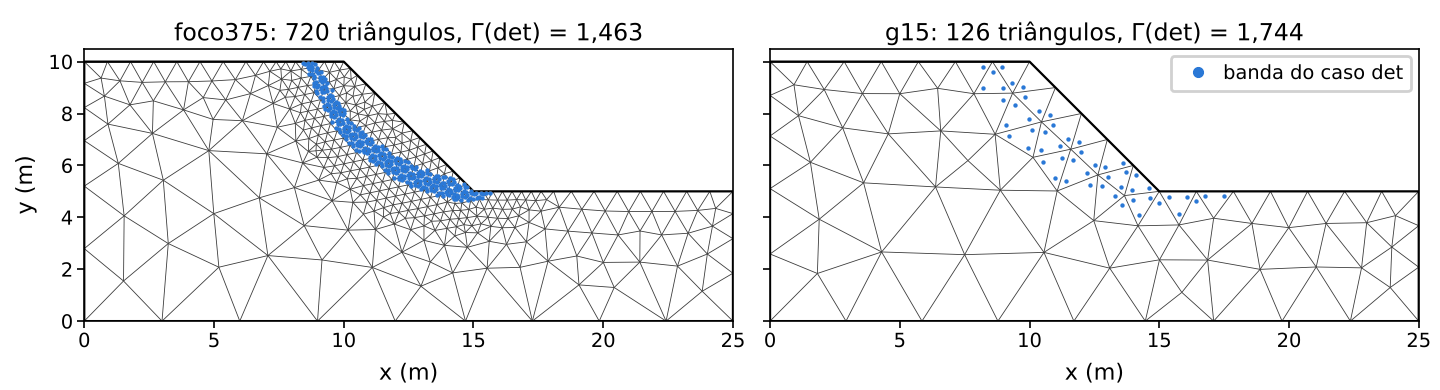
\includegraphics[width=\textwidth]{figuras/niv_malhas_iniciais.png}
  \caption{Malhas iniciais (etapa~1) do estudo de níveis: foco375 (720 triângulos; $h = 0{,}375$~m
    na faixa em torno das bandas de um estudo anterior, Figura~\ref{fig:ref:malhas_fixas}) e g15
    (126 triângulos; o mesmo contorno sem o foco, só com 1,5~m perto da superfície e até 3~m no
    interior). Em azul, a banda de ruptura do caso determinístico obtida em cada uma (pontos de
    integração com $\sqrt{J_2}$ da deformação plástica $\geq 0{,}1$ do máximo no instante do fator),
    que guia o refino; $\Gamma(\mathrm{det}) = 1{,}463$ na foco375 e $1{,}744$ na g15.}
  \label{fig:niv:malhas_iniciais}
\end{figure}

\begin{figure}[htbp]
  \centering
  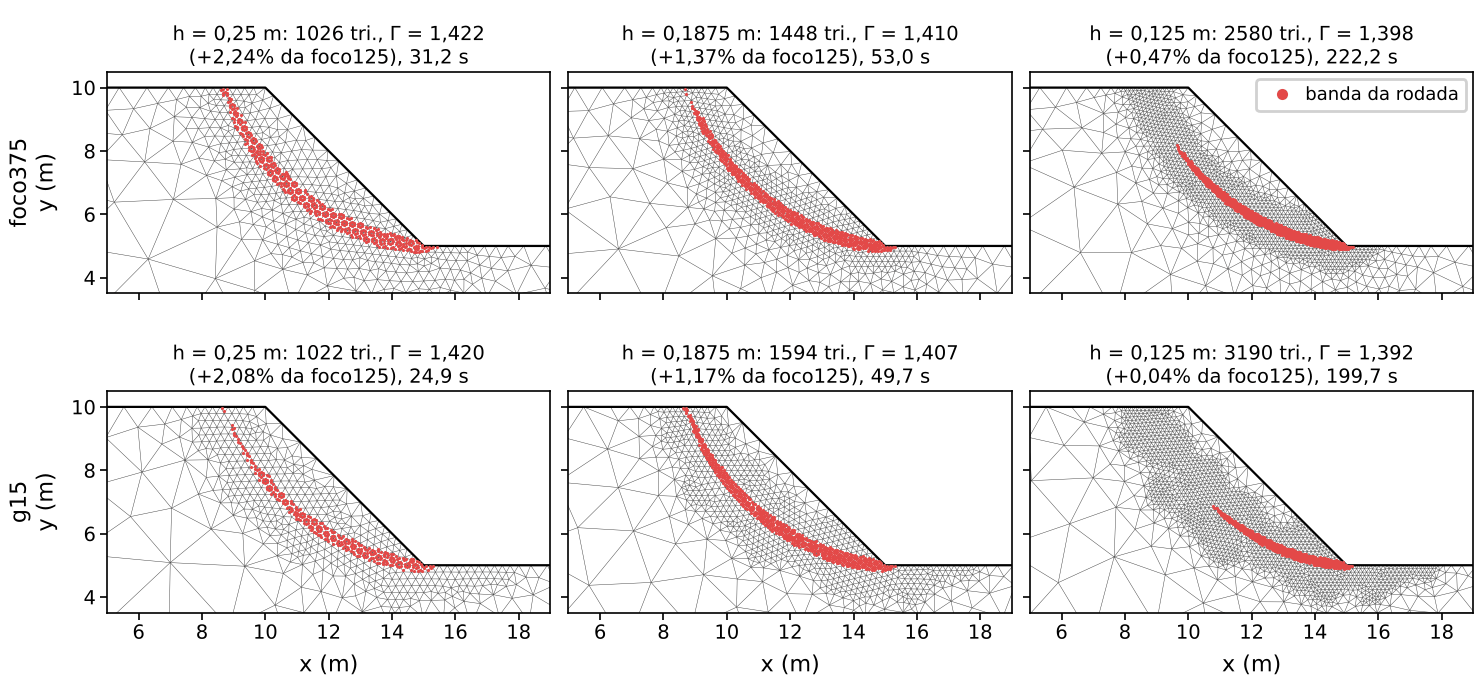
\includegraphics[width=\textwidth]{figuras/niv_niveis_det.png}
  \caption{Níveis de refinamento num passo, caso determinístico. Linhas: malha inicial (foco375,
    g15); colunas: tamanho $h$ dos elementos em torno da banda da etapa~1 (0,25, 0,1875 e
    0,125~m, sempre até 0,375~m dos pontos da banda). Cada painel mostra a malha refinada,
    ampliada na região do talude, e a banda da sua rodada (em vermelho, mesma definição da
    Figura~\ref{fig:niv:malhas_iniciais}). Títulos: triângulos, $\Gamma$, diferença relativa ao
    $\Gamma$ da malha fixa foco125 ($1{,}391$) e tempo de CPU da cadeia (etapa~1 + geração da
    malha + rodada refinada). Na foco375, a coluna $h = 0{,}125$~m é a malha refinada da comparação
    (Figura~\ref{fig:ref:metodo_det}), rodada com 2 processos simultâneos (3 no estudo de níveis).}
  \label{fig:niv:niveis_det}
\end{figure}

\begin{figure}[htbp]
  \centering
  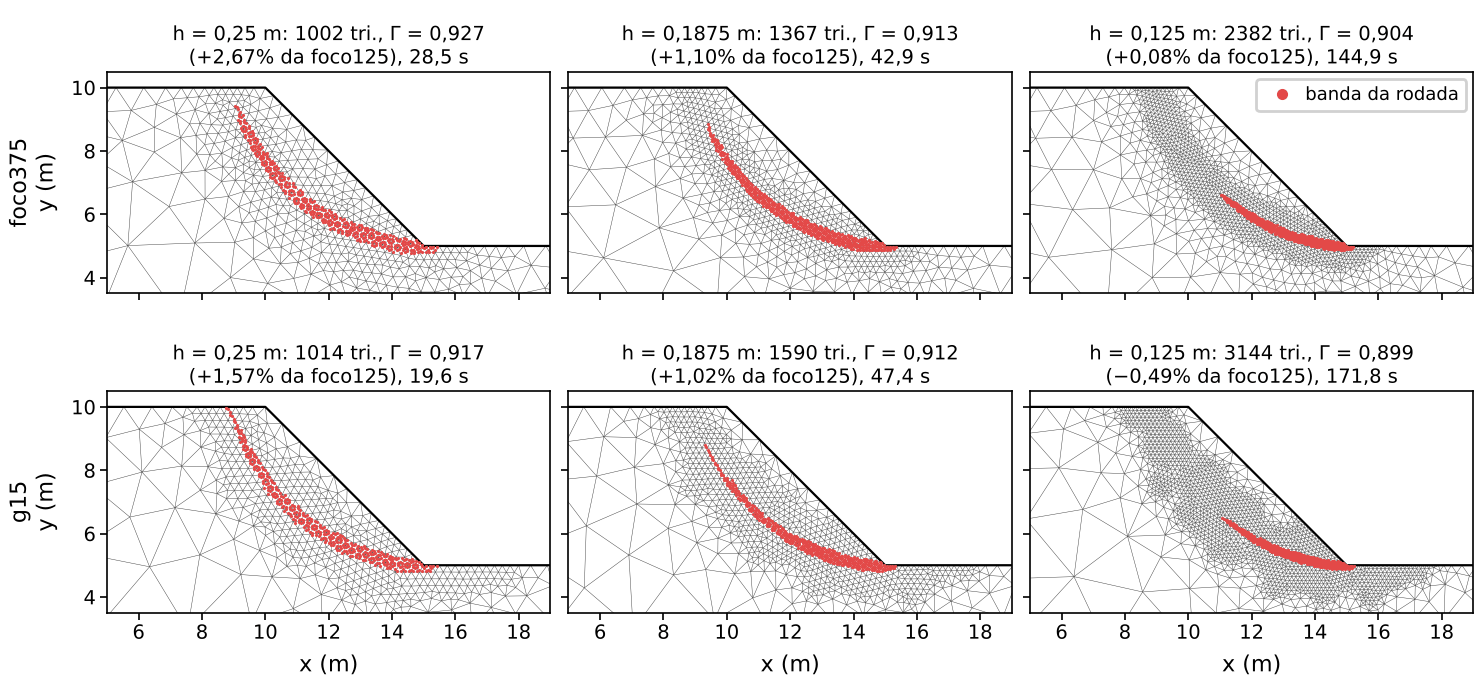
\includegraphics[width=\textwidth]{figuras/niv_niveis_r00005.png}
  \caption{Como na Figura~\ref{fig:niv:niveis_det}, para a realização r5, a de menor $\Gamma$
    ($0{,}903$ na foco125).}
  \label{fig:niv:niveis_r5}
\end{figure}

\begin{figure}[htbp]
  \centering
  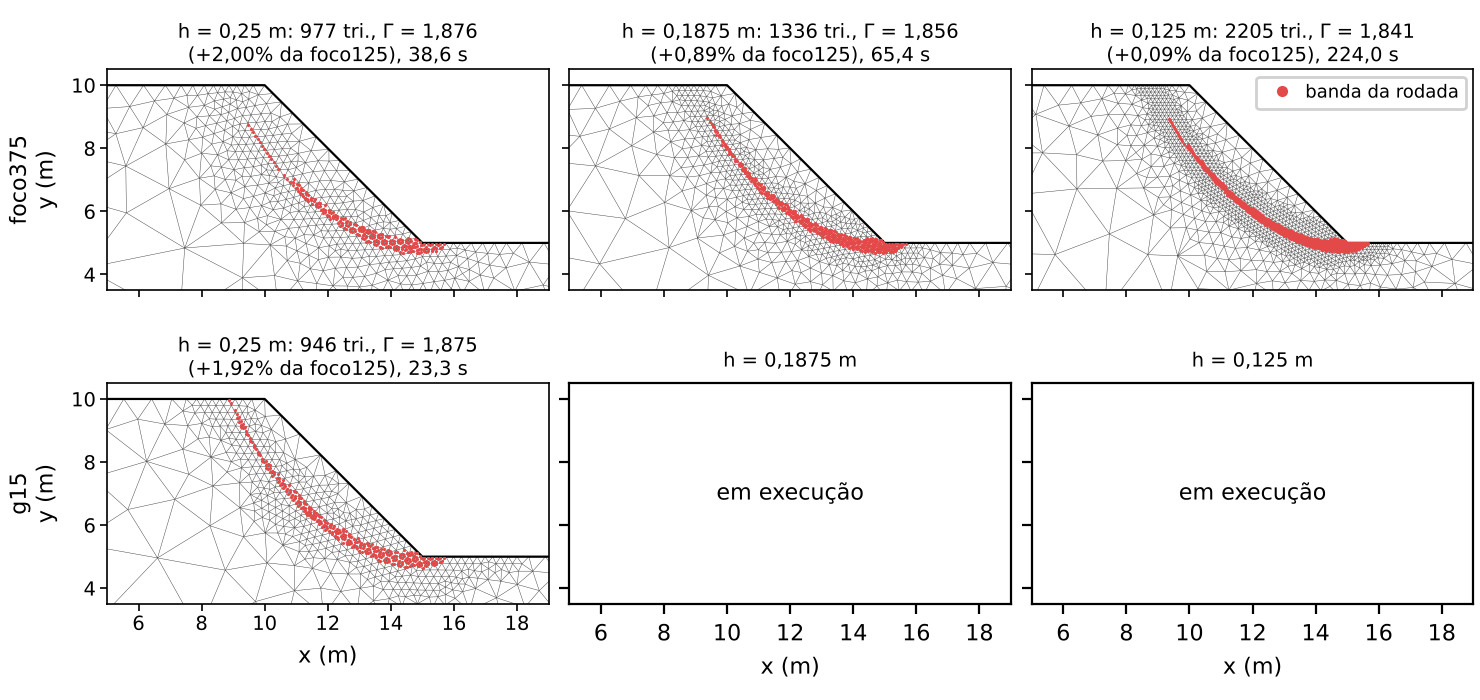
\includegraphics[width=\textwidth]{figuras/niv_niveis_r00003.png}
  \caption{Como na Figura~\ref{fig:niv:niveis_det}, para a realização r3, a de maior $\Gamma$
    ($1{,}840$ na foco125).}
  \label{fig:niv:niveis_r3}
\end{figure}

\begin{figure}[htbp]
  \centering
  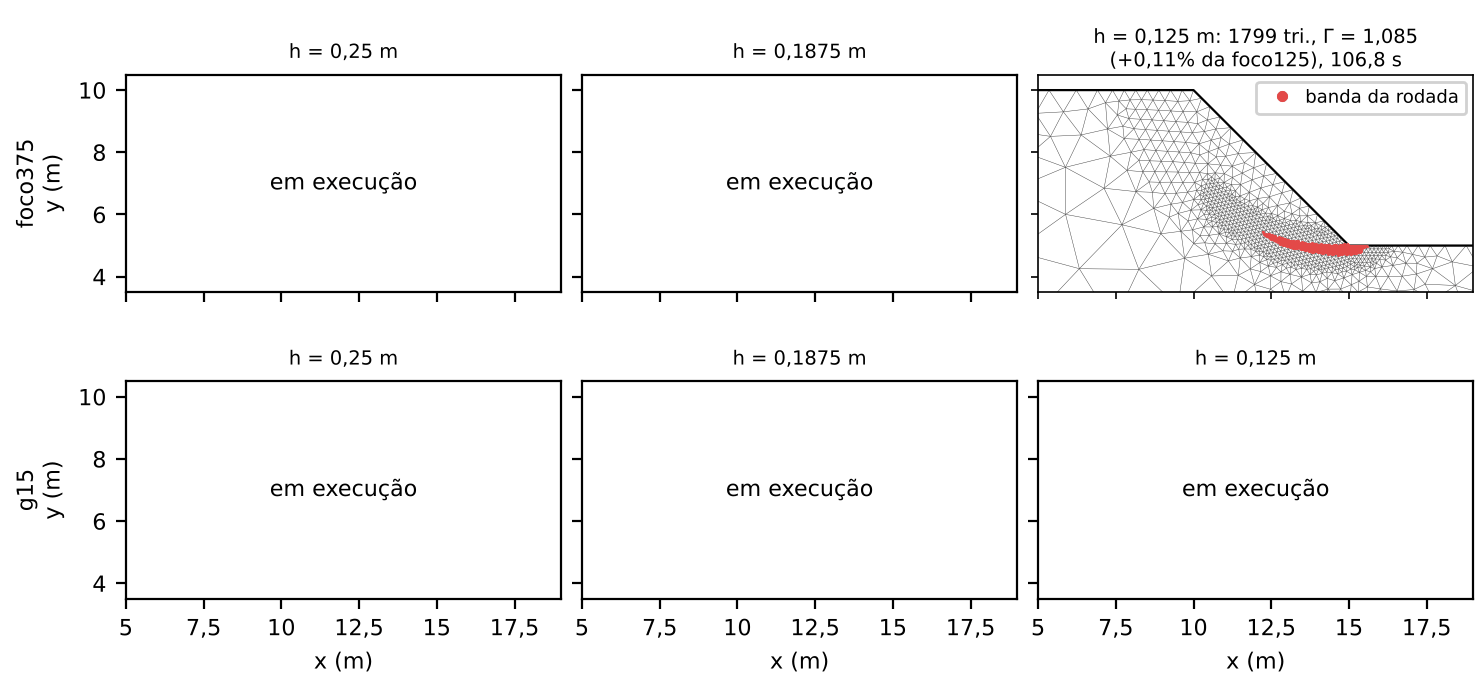
\includegraphics[width=\textwidth]{figuras/niv_niveis_r00007.png}
  \caption{Como na Figura~\ref{fig:niv:niveis_det}, para a realização r7 ($\Gamma = 1{,}084$ na
    foco125), cuja banda fica junto ao pé do talude.}
  \label{fig:niv:niveis_r7}
\end{figure}
}{}
